\documentclass{amsart}
%\documentclass[a4paper,10pt]{scrartcl}

\usepackage[utf8x]{inputenc}
\usepackage[british]{babel}
%\usepackage[a4paper, inner=0.5cm, outer=0.5cm, top=1cm,
%bottom=1.5cm, bindingoffset=1cm]{geometry}
\usepackage{amsmath}
\usepackage{amssymb, latexsym}
\usepackage{longtable}
\usepackage[table]{xcolor}
\usepackage{textcomp} 
\usepackage{stmaryrd}
\usepackage{graphicx}
\usepackage{enumitem}
\usepackage{yfonts}
\usepackage{algpseudocode}
\usepackage{algorithm}
\usepackage{hyperref}
\usepackage{MnSymbol}

\setlist[enumerate]{label*=\arabic*.}
\newtheorem{theorem}{Theorem}[section]
\newtheorem{example}{Example}[section]
\newtheorem{definition}{Definition}[section]
\newtheorem{proposition}{Proposition}[section]
\newtheorem{notation}{Notation}[section]

\renewcommand{\algorithmicrequire}{\textbf{Input:}}
\renewcommand{\algorithmicensure}{\textbf{Output:}}

\title{Why does the OWL Reasoner ignore my Constraint?}
\author{Henriette Harmse}
\date{\today}

\pdfinfo{%
  /Title    (Why does the OWL Reasoner ignore my Constraint?)
  /Author   (Henriette Harmse)
  /Creator  ()
  /Producer ()
  /Subject  (DL)
  /Keywords ()
}

\begin{document}
  \maketitle
  
  
  A most frustrating problem often encountered by people, with experience in relational databases when they are introduced to OWL ontologies, is that OWL ontology reasoners seem to ignore constraints. In this post I give examples of this problem, explain why they happen and I provide ways to deal with each example. 
  
  \section{An Example}
  A typical example encountered in relational databases is that of modeling orders with orderlines, which can be modeled via \texttt{Orders} and \texttt{Orderlines} tables where the \texttt{Orderlines} table has a foreign key constraint to the \texttt{Orders} table. A related OWL ontology is given in Figure~\ref{f_Order}. It creates as expected \texttt{Order} and \texttt{Orderline} classes with a \texttt{hasOrder} object property. That individuals of \texttt{Orderline} are necessarily associated with \textbf{one} order is enforced by \texttt{Orderline} being a subclass of \texttt{hasOrder exactly 1 owl:Thing}. 
  
    \begin{figure}
      %trim option's parameter order: left bottom right top
      \centering 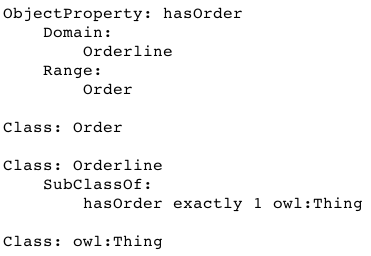
\includegraphics[trim = 0mm 0mm 0mm 0mm, clip, scale=0.5]{./Order.png}
      \vspace{-3mm}
      \caption{An ontology modeling orders and orderlines}\label{f_Order}
    \end{figure}
    
  \section{Two Problems}
  Two frustrating and most surprising errors given the Order ontology are: (1) if an \texttt{Orderline} individual is created for which no associated \texttt{Order} individual exists, the reasoner will not give an inconsistency, and (2) if an \texttt{Orderline} individual is created for which two or more \texttt{Order} individuals exist, the reasoner will also not give an inconsistency.
  
  \subsection{Missing Association Problem}
  Say we create an individual \texttt{orderline123} of type \texttt{Orderline}, which is not associated with an individual of type \texttt{Order}, in this case the reasoner will not give an inconsistency. The reason for this is due to the \textbf{open world assumption}. Informally it means that the only inferences that the reasoner can make from an ontology is based on explicit information stated in the ontology or what can derived from explicit stated information. 
  
  When you state \texttt{orderline123} is an \texttt{Orderline}, there is \textbf{no explicit information} in the ontology that states that \texttt{orderline123} is \textbf{not} associated with an individual of \texttt{Order} via the \texttt{hasOrder} property. To make explicit that \texttt{orderline123} is not in such a relation, you have to define \texttt{orderline123} as in Figure~\ref{f_HasNoOrder}. \texttt{hasOrder max 0 owl:Thing} states that it is known that \texttt{orderline123} is not associated with an individual via the \texttt{hasOrder} property.
 
    \begin{figure}
      %trim option's parameter order: left bottom right top
      \centering 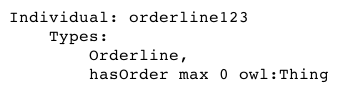
\includegraphics[trim = 0mm 0mm 0mm 0mm, clip, scale=0.5]{./HasNoOrder.png}
      \vspace{-3mm}
      \caption{Enforcing that \texttt{orderline123} is not associated via \texttt{hasOrder}}\label{f_HasNoOrder}
    \end{figure}
    
  \subsection{Too Many Associated Individuals Problem}
  Assume we now change our definition of our \texttt{orderline123} individual to be associated via \texttt{hasOrder} to two individuals of \texttt{Order} as shown in Figure~\ref{f_HasTwoOrders}. Again, most frustratingly the reasoner does not find that the ontology is inconsistent. The reason for this is that OWL does not make the \textbf{unique name assumption}. This means that individuals with different names can be assumed by the reasoner to represent a single individual. To force the reasoner to see \texttt{order1} and \texttt{order2} as necessarily different, you can state \texttt{order1} different from \texttt{order2} by adding \texttt{DifferentFrom:order2} to \texttt{order1} (or similarly for \texttt{order2}).

     \begin{figure}
      %trim option's parameter order: left bottom right top
      \centering 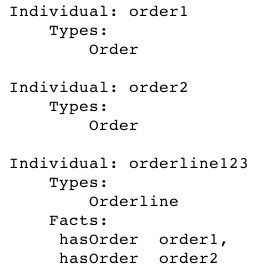
\includegraphics[trim = 0mm 0mm 0mm 0mm, clip, scale=0.5]{./HasTwoOrders.png}
      \vspace{-3mm}
      \caption{\texttt{orderline123} associated with two individuals of type \texttt{Order}}\label{f_HasTwoOrders}
    \end{figure}
    
  \section{Constraint Checking versus Deriving Inferences}
  The source of the problems described here is due to the difference between the purposes of a relational database and an OWL reasoner. The main purpose of a relational database is to enable view and edit access of the data in such a way that the integrity of the data is maintained. A relational database will ensure that the data adheres to the constraints of its schema, but it cannot make any claims beyond what is stated by the data it contains. The main purpose of an OWL reasoner is to derive inferences from statements and facts. As an example, from the statement \texttt{Class: Dog SubclassOf: Animal} and the fact \texttt{Individual: pluto Type: Dog} it can be derived that \texttt{pluto} is an \texttt{Animal}, even though  the ontology nowhere states explicitly that \texttt{pluto} is an \texttt{Animal}.
    
  \section{Conclusion}
  Many newcomers to OWL ontologies get tripped up by the difference in purpose of relational databases and OWL ontologies. In this post I explained some of the challenges that stem from this difference in purpose and how to deal with them. 
  
  
  \bibliographystyle{amsplain}
  \bibliography{../../../BibliographicDetails_v.0.1}
 
\end{document}
